%%%%%%%%%%%%%%%%%%%%%%%%%%%%%%%%%%%%%%%%%%%%%%%%%%%%%%%%%%%%%%%%%%%%%%%%
%     LaTeX source code to approximate a Draft NIST Technical report
%	  Instructions for authors: tinyurl.com/techpubsnist 
%	DOI watermark will be added on final PDF
% 	Developed by K. Miller, kmm5@nist.gov 
%	Last updated: 22-March-2019
%%%%%%%%%%%%%%%%%%%%%%%%%%%%%%%%%%%%%%%%%%%%%%%%%%%%%%%%%%%%%%%%%%%

%%%%%%%%%%%%%%%%%%%%%%
% Template further altered by Armen Amirkhanian
% for use with UA lab courses in an effort to 
% have a standardized format for lab documents
% Last update 9-April-2020
%
% TODO:
% --Get the appendices to dynamically link, tocloft causes problems
%%%%%%%%%%%%%%%%%%%%%%

\documentclass[12pt]{article}
\usepackage{amsmath}
\usepackage{amsfonts}   % if you want the fonts
\usepackage{amssymb}    % if you want extra symbols
\usepackage{graphicx}   % need for figures
\usepackage{xcolor}
\usepackage{bm}
\usepackage{secdot}		
\usepackage{mathptmx}
\usepackage{float}
\usepackage[utf8]{inputenc}
\usepackage{textcomp}
\usepackage[hang,flushmargin,bottom]{footmisc} % footnote format
\usepackage{xspace}
%\usepackage{lineno}
\usepackage{ragged2e}
\usepackage{parskip}
\usepackage{textcomp}

\usepackage{tikz}
\usetikzlibrary{shapes.geometric, arrows}
\tikzstyle{startstop} = [rectangle, rounded corners, minimum width=2cm, minimum height=1cm,text centered, draw=black, fill=red!20]
\tikzstyle{arrow} = [thick,->,>=stealth]

\usepackage{titlesec}
\titleformat{\section}{\normalsize\bfseries}{\thesection.}{1em}{}	% required for heading numbering style
\titleformat*{\subsection}{\normalsize\bfseries}

\usepackage{tocloft}	% change typeset, titles, and format list of appendices/figures/tables
\renewcommand{\cftdot}{}	
\renewcommand{\contentsname}{Table of Contents}
\renewcommand{\cftpartleader}{\cftdotfill{\cftdotsep}} % for parts
\renewcommand{\cftsecleader}{\cftdotfill{\cftdotsep}}
\renewcommand\cftbeforesecskip{\setlength{4pt}{}}
\addtolength{\cftfignumwidth}{1em}
\renewcommand{\cftfigpresnum}{\figurename\ }
\addtolength{\cfttabnumwidth}{1em}
\renewcommand{\cfttabpresnum}{\tablename\ }
\setlength{\cfttabindent}{0in}    %% adjust as you like
\setlength{\cftfigindent}{0in} 

\usepackage{enumitem}         % to control spacing between bullets/numbered lists

\usepackage[numbers,sort&compress]{natbib} % format bibliography 
\renewcommand{\bibsection}{}
\setlength{\bibsep}{0.0pt}

\usepackage[hidelinks]{hyperref}
\hypersetup{
	colorlinks = true,
urlcolor ={blue},
citecolor = {.},
linkcolor = {.},
anchorcolor = {.},
filecolor = {.},
menucolor = {.},
runcolor = {.}
pdftitle={},
pdfsubject={},
pdfauthor={},
pdfkeywords={}
}
\urlstyle{same}

\usepackage{epstopdf} % converting EPS figure files to PDF

\usepackage{fancyhdr, lastpage}	% formatting document, calculating number of pages, formatting headers
\setlength{\topmargin}{-0.5in}
\setlength{\headheight}{39pt}
\setlength{\oddsidemargin}{0.25in}
\setlength{\evensidemargin}{0.25in}
\setlength{\textwidth}{6.0in}
\setlength{\textheight}{8.5in}

\usepackage{caption} % required for Figure labels
\captionsetup{font=small,labelfont=bf,figurename=Fig.,labelsep=period,justification=raggedright} 

%%%%%%%%%%% !!!!!REQUIRED - FILL OUT METADATA HERE !!!!!!!! %%%%%%%%%%%%%%
%%%%%%%%%%%%%%%%%%%%%%%%%%%%%%%%%%%%%%%%%%%%%%%%%%%%%%%%%%%%%%%%%%%%%%%%%%
\newcommand{\CourseNum}{CE340}
\newcommand{\CourseName}{Geotechnical Engineering}
\newcommand{\LabTitle}{Sand Cone}
\newcommand{\LastUpdate}{Summer 2020}

%%%%%%%%%%%%%%%%%%%%%%%%%%%%%%%%%%%%%%%%%%%%%%%%%%%%%%%%%%%%%%%%%%%%
%   	BEGIN DOCUMENT 
%%%%%%%%%%%%%%%%%%%%%%%%%%%%%%%%%%%%%%%%%%%%%%%%%%%%%%%%%%%%%%%%%%%%
\begin{document}
	\urlstyle{rm} % Format style of \url   
%\linenumbers
\begin{titlepage}
\begin{flushright}
\LARGE{\textbf{\CourseNum{} -- \CourseName}}\\
\vfill
\Huge{\textbf{\LabTitle}}\\
    \vfill
%%%%%%%%%%%%%%%%%%%%%%%%%%%%%%%%%%%%%%%%%%%%%%%%%%%%%%%%%%%%%%%%%%%%
%	Authors - add complete list of authors, affiliations will be 
%   added on title page
%%%%%%%%%%%%%%%%%%%%%%%%%%%%%%%%%%%%%%%%%%%%%%%%%%%%%%%%%%%%%%%%%%%%
    \large Dr. Armen Amirkhanian, P.E.\\
\vfill
%%%%%%%%%%%%%%%%%%%%%%%%%%%%%%%%%%%%%%%%%%%%%%%%%%%%%%%%%%%%%%%%%%%%
%	The DOI is automated based on metadata.	
%%%%%%%%%%%%%%%%%%%%%%%%%%%%%%%%%%%%%%%%%%%%%%%%%%%%%%%%%%%%%%%%%%%%
\normalsize This work is licensed under the Creative Commons Attribution-ShareAlike 4.0 International License. To view a copy of this license, visit:
\href{http://creativecommons.org/licenses/by-sa/4.0/}{http://creativecommons.org/licenses/by-sa/4.0/}.


\includegraphics[width=0.07\textwidth]{cc.eps}
\includegraphics[width=0.07\textwidth]{by.eps}

\includegraphics[width=0.07\textwidth]{sa.eps}
\vfill


\includegraphics[width=0.3\linewidth]{Logo.eps}\\ 
 
  
\end{flushright}
\end{titlepage}

\begin{titlepage}
\begin{center}
\normalsize 
Certain commercial entities, equipment, or materials may be identified in this document in order to describe an experimental procedure or concept adequately. Such identification is not intended to imply recommendation or endorsement by The University of Alabama or the listed authors, nor is it intended to imply that the entities, materials, or equipment are necessarily the best available for the purpose.\\

\vfill
Any opinions or recommendations are solely those of the authors and do not represent the official view or policy of The University of Alabama.
\end{center}
\begin{flushright}
\vfill
\normalsize 
This document was last updated in \textbf{\LastUpdate} and should contain \textbf{\pageref{LastPage}} pages of content exclusive of these title pages, abstract, and other front matter. If the document appears to be incomplete, please contact the author(s).\\
\vfill
One man’s magic is another man’s engineering\\
\textit{Robert Heinlein}
\end{flushright}
\end{titlepage}
%%%%%%%%%%%%%%%%%%%%%%%%%%%%%%%%%%%%%%%%%%%%%%%%%%%%%%%%%%%%%%%%%%%%
%   Start front matter - page number starts with "i"
%%%%%%%%%%%%%%%%%%%%%%%%%%%%%%%%%%%%%%%%%%%%%%%%%%%%%%%%%%%%%%%%%%%%
\pagenumbering{roman}
\section*{Abstract}
\normalsize The evaluation of compaction in the field is a critical component to many construction processes. There are numerous technologies available to assess the \textit{in-situ} density of soils including, but not limited to sand cone, balloon, nuclear density gauge, and others. Out of these, the sand cone is the simplest, and perhaps oldest, test method. A hole is dug at the area of interest and the removed material is weighed. Then the hole is filled carefully with a sand of known density. The amount of sand needed to fill the hole is calculated and from this, the volume is determined. Knowing the weight of material removed to create the hole and the volume of the hole, the unit weight, and thus the compaction, can be calculated.\\

\vfill
\section*{Keywords}
\normalsize compaction; sand cone; field density.\\
\pagebreak
%%%%%%%%%%%%%%%%%%%%%%%%%%%%%%%%%%%%%%%%%%%%%%%%%%%%%%%%%%%%%%%%%%%%
%   Table of Contents is required
% 	List of Tables & Figures required if more than 5 tables/figures
%%%%%%%%%%%%%%%%%%%%%%%%%%%%%%%%%%%%%%%%%%%%%%%%%%%%%%%%%%%%%%%%%%%%
\begin{center}
\tableofcontents
\pagebreak
\listoftables
\listoffigures
\end{center}
\pagebreak
\section*{Required Specifications}
The following specifications are required to complete this laboratory exercise:
\begin{description}
\item[ASTM D1556] Standard Test Method for Density and Unit Weight of Soil in Place by Sand-Cone Method
\end{description}

The following specifications are optional, but they are listed here in the event more information is needed to complete the laboratory exercise:
\begin{description}
\item[ASTM D698] Test Methods for Laboratory Compaction Characteristics of Soil Using Standard Effort (12,400 ft-lbf/ft$^3$ (600 kN-m/m$^3$))
\item[ASTM D6026] Standard Practice for Using Significant Digits in Geotechnical Data
\item[ASTM E11] Specification for Woven Wire Test Sieve Cloth and Test Sieves
\end{description}
\pagebreak
%%%%%%%%%%%%%%%%%%%%%%%%%%%%%%%%%%%%%%%%%%%%%%%%%%%%%%%%%%%%%%%%%%%%
%   Start body of text - page number starts with "1"
%%%%%%%%%%%%%%%%%%%%%%%%%%%%%%%%%%%%%%%%%%%%%%%%%%%%%%%%%%%%%%%%%%%%
\section{Sand Cone}
\label{sec:intro}
\pagenumbering{arabic}
\normalsize 
The sand cone test has been around for over 60 years. It is a reliable and straightforward method to measure unit weight in the field. This is an in-situ\footnote{This means ``in place'' or at the original location, that is, not bringing it back to the lab.} test method. While not a common test nowadays, as there are faster test methods available to determine the unit weight of a soil in the field, the sand cone remains a practical method that has no moving parts, batteries, or radioactive sources to maintain. Additionally, it is easy to see visually what is being measured.

\subsection{Objectives}
\label{ssec:headingscap}
At the completion of this lab exercise, you will have satisfied the following objectives:
\begin{enumerate}
    \item Perform a calibration procedure for the sand cone equipment
    \item Perform a field unit weight measurement using the sand cone method
    \item Perform calculations necessary to determine the field unit weight
\end{enumerate}

\subsection{Learning Outcomes}
At the completion of this lab exercise, you should be able to:
\begin{itemize}
    \item understand an ASTM calibration process
    \item perform calculations necessary to determine the field unit weight from sand cone data
    \item understand the concept of compaction percentage
\end{itemize}

\pagebreak
\subsection{Procedure}
The sand cone test procedure is divided into four parts: calibration, preparation, execution, and analysis. ASTM D1556 will be used for the calibration and procedure methods. Up to this point, we have largely ignored the calibration procedures in ASTM standard for our test methods. However, in the case of the sand cone test, it is extremely important and is done more often than with other testing procedures. The calibration will take place in the laboratory while the actual measurement will be conducted in the field.

\subsubsection{Calibration}
There are two steps to the calibration process but you will only be conducting the first step. The second step is described in ASTM D1556 \S A.2 and determines the unit weight of the sand used for the sand cone. This unit weight will be provided to you. You will generally follow the steps outlined in ASTM D1556 \S A.1. There are two methods listed but they are nearly identical. The second method simply outlines a procedure for multiple sand cone sets.

Following the procedures outlined for Method A in ASTM D1556 \S A1.2.3, you will set the base plate on the laboratory table and then weigh the sand cone apparatus. Then, place the sand cone in the base plate and open the valve and allow sand to fill the cone portion and the gap between the cone and table. After the sand stops following, you will close the valve and slowly remove the cone. You will then weigh the sand cone apparatus (which now has less sand in it). Finally, you will carefully scoop/sweep the sand into a container for reuse\footnote{ASTM D1556 generally discourages reuse of the sand but we will be careful not to contaminate it}. Using the provided unit weight of the sand, you can easily calculate the volume of the cone and gap by using the difference in weights. This value will be your cone correction factor.

\subsubsection{Preparation}
You will need five pieces of equipment for this procedure: sand cone apparatus, base plate, scoop, sample container, and a scale\footnote{We will not bring this into the field; we will bring the soil sample back to the lab to weigh.}. Ensure the sand cone apparatus is filled with enough sand and obtain the filled weight of the apparatus. Finally, obtain the empty weight of the sample container.

\subsubsection*{Preparation Checklist}
\begin{itemize}
    \item Obtain sand cone apparatus and base plate
    \item Obtain scoop and sample container
    \item Obtain the filled weight of the apparatus
    \item Obtain the empty weight of the sample container
\end{itemize}

\subsubsection{Execution}
The execution process is straightforward. You will go to the designated site and set your base plate down. Hammer the soil stakes in to stabilize the base plate while you excavate the soil with the scoop. It is critical that as you scoop soil out to form a hole that you do not lose any soil. All of the excavated soil should be placed in the sample container and sealed until you can obtain the in-situ mass back in the lab.

The minimum size of the hole is listed in ASTM D1556 \S7.1.5 and is dependent on the gradation of the soil you are testing. Essentially, we want a hole big enough to reduce error but smaller than the volume of sand in our sand cone. The shape of the hole you dig is also important as we need the sand to freely flow and fill in the hole. We cannot have overhangs or crevices that the sand would not easily reach (Fig. \ref{fig:hole_cross_section}).

\begin{figure}[H]
    \centering
    
\includegraphics[width=0.8\textwidth]{hole_cross_section.png}
    \caption{Example hole cross sections with (A) and (B) indicating good holes and (C) and (D) indicating poor holes.}
    \label{fig:hole_cross_section}
\end{figure}

After you have collected all of the loose soil in the sample container, seal it to prevent moisture loss while you complete the sand cone test. Place the sand cone apparatus on top of the base plate and ensure it is fully seated. Open the valve and allow the sand to fill the entire volume. Once the sand has stopped flowing, close the valve and slowing remove the sand cone apparatus. As previously mentioned, we generally cannot reuse the sand because it becomes contaminated with the soil we are testing on. Thus, you will leave the sand in the hole and remove the stakes and base plate for transport back to the lab.

Once back in the lab, obtain the weights of the soil sample and the emptied sand cone apparatus. Your soil sample will be oven dried and the resulting oven dry mass will be provided to you. Ensure your sample container is sufficiently labeled for later identification.

\subsubsection*{Execution Checklist}
\begin{itemize}
    \item Excavate a hole and collect all soil in a sealed container
    \item Weigh sample container with moist soil sample
    \item Weigh emptied sand cone apparatus
    \item Place sample container in drying oven
\end{itemize}

\subsubsection{Analysis}
The calculations for determining the densities is straightforward and clearly outlined in ASTM D1556 \S8. We first calculate the volume of the hole. This is done by taking the difference of the starting weight and ending weight of the sand cone apparatus, subtracting the calibration value determined earlier, and then dividing by the unit weight of the sand. Keep track of your units!

After the volume is known, the calculation of both wet and dry densities is easily performed. It is simply the measured wet or dry weight of the soil removed from the hole divided by the volume of the hole. The number of decimal places we can report to is outlined in ASTM D1556 \S9.4.

The last thing we need to do with our data is to see at what ``percent compaction'' we were at in the field. When we run a density check in the field, we are trying to see if we have reached some target compaction. It is most commonly reported as a percentage of the maximum dry density, which was determined in the lab from the standard Proctor test following ASTM D698. For example, let's assume our specimen has a maximum dry density, determined from the standard Proctor, of 125 lbs/ft$^3$. If the results of our sand cone test determine that the in-situ dry density is 121 lbs/ft$^3$, we have obtained 96.8\% compaction. The required percentage depends on the project details, but minimum compaction values of 90\% or 95\% are most common.

\subsubsection*{Analysis Checklist}
\begin{itemize}
    \item Calculate the volume of the hole
    \item Calculate dry mass of soil removed
    \item Calculate in-situ wet density
    \item Calculate in-situ dry density
    \item Calculate in-situ percent compaction
\end{itemize}

\subsection{Summary}
You have successfully run a sand cone test. As you likely noticed, the process is relatively straightforward and easy to run. This test used to be a routine test but was surpassed by faster and more accurate methods such as nuclear density gauges. Even though not as common, the sand cone method provides a good opportunity to visually observe how the compaction can be measured and more importantly, the size of the measurement.



%\section*{References}
%\addcontentsline{toc}{section}{References}
%\bibliographystyle{techpubs}
%\bibliography{References}

%%%%%%%%%%%%%%%%%%%%%%%%%%%%%%%%%%%%%%%%%%%%%%%%%%%%%%%%%%%%%%%%%%%%
%   Please use the techpubs BibTeX style when compiling bibliography, or follow the instructions on tinyurl.com/techpubsnist to format your .bib / .bbl file appropriately.
%%%%%%%%%%%%%%%%%%%%%%%%%%%%%%%%%%%%%%%%%%%%%%%%%%%%%%%%%%%%%%%%%%%%
%\pagebreak

%\section*{Appendix A: Example Gradation Worksheet}
%\label{AppendixA}
%\addcontentsline{toc}{section}{Appendix A: Example Gradation Worksheet}
%\begin{center}
%    \includegraphics[width=1\linewidth]{Example_Sieve_Analysis_Worksheet.eps}
%\end{center}

%\pagebreak
%\section*{Appendix B: Change Log}
%\addcontentsline{toc}{section}{Appendix B: Change Log}
%This document was originally created on April 16, 2020. Any changes will be documented in this appendix.

\end{document}
%%%%%%%%%%%%%%%%%%%%%%%%%%%%%%%%%%%%%%%%%%%%%%%%%%%%%%%%%%%%%%%%%%%%
%   When referring to references in the text parenthetically, 
%	use the form “[1].” For example, “As Jones and Smith have shown [1];”
%	 however, when a reference is referred to non-parenthetically, use the form 
%	“. . . Ref. [1] . . .” (except at the beginning of a sentence where
%	“Reference [1] . . .” is the correct form).
%%%%%%%%%%%%%%%%%%%%%%%%%%%%%%%%%%%%%%%%%%%%%%%%%%%%%%%%%%%%%%%%%%%%

%%%%%%%%%%%%%%%%%%%%%%%%%%%%%%%%%%%%%%%%%%%%%%%%%%%%%%%%%%%%%%%%%%%%
%   Section references are “Sec. X”.
% 	“Section X” is used at beginning of sentence. 
%%%%%%%%%%%%%%%%%%%%%%%%%%%%%%%%%%%%%%%%%%%%%%%%%%%%%%%%%%%%%%%%%%%%

%%%%%%%%%%%%%%%%%%%%%%%%%%%%%%%%%%%%%%%%%%%%%%%%%%%%%%%%%%%%%%%%%%%%
%   Equation references are “Eq. (X)”.
% 	“Equation (1) is used at beginning of sentence.
%	Equations are numbered (#) on the right, per the standard LaTeX format
%%%%%%%%%%%%%%%%%%%%%%%%%%%%%%%%%%%%%%%%%%%%%%%%%%%%%%%%%%%%%%%%%%%%

%%%%%%%%%%%%%%%%%%%%%%%%%%%%%%%%%%%%%%%%%%%%%%%%%%%%%%%%%%%%%%%%%%%%
%   Tables should appear after they are mentioned in the text. 
%	Superscripted letters (a, b, c, etc.) should be used for table footnotes.
%%%%%%%%%%%%%%%%%%%%%%%%%%%%%%%%%%%%%%%%%%%%%%%%%%%%%%%%%%%%%%%%%%%%

%%%%%%%%%%%%%%%%%%%%%%%%%%%%%%%%%%%%%%%%%%%%%%%%%%%%%%%%%%%%%%%%%%%%
%   Figure references are “Fig. X”.
% 	“Figure X” is used at beginning of sentence. 
% 	Figures should appear after they are mentioned in the text.
%	Figures must have embedded alternate text or “alt text” in order 
%	to comply with Section 508 accessibility standards. 
%%%%%%%%%%%%%%%%%%%%%%%%%%%%%%%%%%%%%%%%%%%%%%%%%%%%%%%%%%%%%%%%%%%%